% ══════════════════════════════════════════════════════════════════
\chapter{Two Collapse Modes: The Empirical Angle Map}
\label{ch:angle_map}
% ══════════════════════════════════════════════════════════════════

\noindent
This chapter provides the most intuitive visualization of why row
centering fails at geometry despite appearing to succeed in PCA plots.

% ──────────────────────────────────────────────────────────────────
\section{Single-Layer Angle Map: All Initializers Are Identical}
\label{sec:single_layer_map}

\subsection{Method}

We generate pairs of random unit vectors at controlled angles
$\alpha \in \{5^\circ, 10^\circ, \dots, 175^\circ\}$ in
$\R^{784}$, pass each pair through one initialized layer followed by
ReLU, and measure the output angle $\alpha'$ between the resulting
vectors.  We average over 200 pairs per angle and 5 random seeds.

\subsection{Results}

\begin{center}
\begin{tabular}{lcc}
\toprule
Initializer & Mean ratio $\alpha'/\alpha$ & Min ratio \\
\midrule
\texttt{he}                          & 0.7751 & 0.5081 \\
\texttt{orthogonal\_he}              & 0.7754 & 0.5081 \\
\texttt{row\_centered\_he\_var\_adj} & 0.7751 & 0.5081 \\
\texttt{kernel\_preserving}          & 0.7772 & 0.5081 \\
\bottomrule
\end{tabular}
\end{center}

All four initializers produce \textbf{identical} single-layer angle
maps (to within measurement noise).  The He empirical result matches
the theoretical prediction from the arc-cosine kernel
(equation~\eqref{eq:angle_map}) to within $0.14^\circ$.

\begin{figure}[h]
\centering
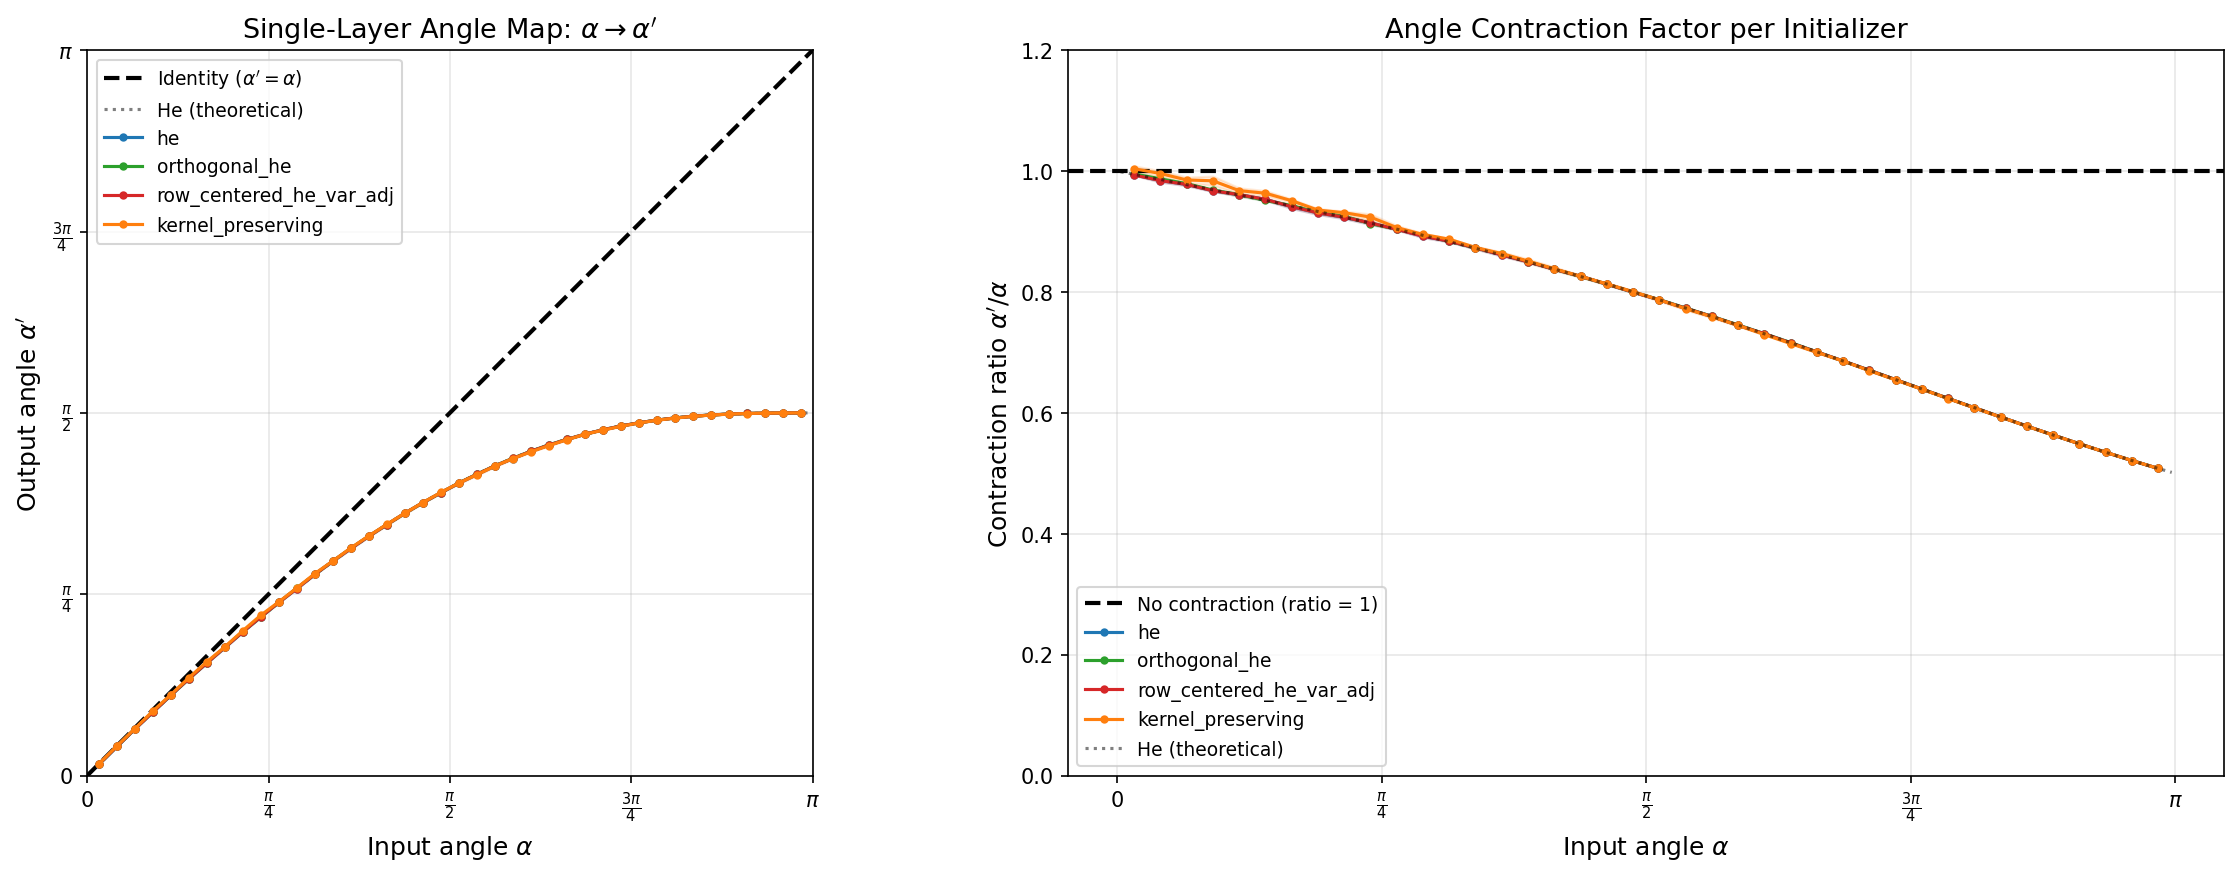
\includegraphics[width=\textwidth]{figures/single_layer_angle_map.png}
\caption{\textbf{Left:} Single-layer angle map $\alpha \to \alpha'$ for
  four initializers (empirical, 200 pairs $\times$ 5 seeds) vs.\ the
  theoretical arc-cosine kernel prediction.
  All initializers lie on top of the theory curve.
  \textbf{Right:} Contraction ratio $\alpha'/\alpha < 1$ for all angles.
  Source: \texttt{notebooks/07\_kernel\_geometry\_analysis.ipynb}, Cell~25.}
\label{fig:single_layer_angle_map}
\end{figure}

\subsection{Why row centering is invisible at one layer}

The experiment uses random \textbf{unit vectors} as inputs.
Unit vectors in high dimensions have near-zero mean:
$\bar{x} = (1/d)\sum_j x_j \approx 0$.  Therefore the DC component
is negligible, and the row centering constraint
$\sum_j W_{ij} = 0$ has almost no effect on the pre-activations
$z_i = \sum_j W_{ij} x_j \approx \sum_j W_{ij}(x_j - \bar{x})$.

\begin{proposition}
For unit vector inputs with zero DC component, the single-layer
angle contraction is determined entirely by the ReLU nonlinearity
(through the arc-cosine kernel $K(\alpha)$), independent of the
weight structure.
\end{proposition}

The differences between initializers emerge only from layer~2 onward,
when the inputs are \emph{post-ReLU activations} with a significant
positive DC component ($\E[a] = \sigma/\sqrt{2\pi} > 0$).

% ──────────────────────────────────────────────────────────────────
\section{Multi-Layer Angle Evolution: Two Different Fixed Points}
\label{sec:two_fixed_points}

\subsection{Method}

Track the angle between a pair of vectors as they propagate through
$L = 20$ layers.  Start from four initial angles:
$\alpha_0 \in \{30^\circ, 60^\circ, 90^\circ, 120^\circ\}$.
Average over 200 pairs and 5 seeds.

\subsection{Results}

\begin{table}[h]
\centering
\begin{tabular}{lcccc}
\toprule
Initializer & $30^\circ \to 20\text{L}$ &
$60^\circ \to 20\text{L}$ &
$90^\circ \to 20\text{L}$ &
$120^\circ \to 20\text{L}$ \\
\midrule
\texttt{he}           & $13.8^\circ$ & $17.4^\circ$ & $18.6^\circ$ & $19.0^\circ$ \\
\texttt{orthogonal\_he} & $12.5^\circ$ & $15.6^\circ$ & $16.8^\circ$ & $17.3^\circ$ \\
\texttt{rc\_var\_adj} & $\bm{70.9^\circ}$ & $\bm{71.3^\circ}$ & $\bm{71.3^\circ}$ & $\bm{71.7^\circ}$ \\
\bottomrule
\end{tabular}
\caption{Output angles after 20 layers.  He converges toward $0^\circ$;
row-centered converges to ${\sim}71^\circ$.}
\label{tab:angle_evolution}
\end{table}

\textbf{He / orthogonal:}
All starting angles contract toward $\bm{0^\circ}$ --- classical
geometric collapse where all representations align
(\emph{identity collapse}).

\textbf{Row-centered:}
All starting angles converge to $\bm{\sim\!71^\circ}$ --- every pair
of points becomes equidistant (\emph{equidistance collapse}).

% ──────────────────────────────────────────────────────────────────
\section{Why $71^\circ$ Is the Row-Centered Fixed Point}
\label{sec:why_71}

\subsection{The mechanism}

\begin{enumerate}
  \item Row centering strips the DC component from post-ReLU
        activations at each layer
        (Proposition~\ref{prop:dc_blind}).
  \item The remaining AC component (directional information) decays
        by $0.826\times$ per layer (equation~\eqref{eq:rc_fwd_gain}).
  \item After enough layers, only random fluctuations from the weight
        matrices remain.
  \item The activations at each layer are non-negative (post-ReLU).
        Random non-negative vectors in high dimension have pairwise
        angles concentrated around a characteristic value determined by
        the geometry of the positive orthant.
\end{enumerate}

\subsection{The positive orthant angle}

For random non-negative vectors $\bm{a}, \bm{b} \in \R_{\geq 0}^d$
with i.i.d.\ entries drawn from a half-Gaussian, the expected cosine
similarity concentrates (for large~$d$) around:
\begin{equation}
  \E\!\left[\frac{\langle \bm{a}, \bm{b} \rangle}
    {\|\bm{a}\| \cdot \|\bm{b}\|}\right]
  \approx \frac{(\E[a_j])^2}{\E[a_j^2]}
  = \frac{1/(2\pi)}{1/2}
  = \frac{1}{\pi}
  \approx 0.318,
\end{equation}
where we used the half-Gaussian moments
(Lemma~\ref{lem:half_gaussian}) with $\sigma^2 = 1$:
$\E[a_j] = 1/\sqrt{2\pi}$, so $(\E[a_j])^2 = 1/(2\pi)$, and
$\E[a_j^2] = 1/2$.
This gives the expected angle:
\begin{equation}\label{eq:fixed_point}
  \alpha^*
  = \arccos\!\left(\frac{1}{\pi}\right)
  \approx 71.5^\circ.
\end{equation}

\begin{remark}
The predicted fixed point ($71.5^\circ$) matches the empirically
observed value ($\sim\!71^\circ$) to within measurement noise.
This excellent agreement confirms the mechanism: after enough layers
of DC stripping and signal decay, the post-ReLU activations become
effectively random non-negative vectors, and their pairwise angles
concentrate at $\arccos(1/\pi)$ --- a universal constant determined
solely by the geometry of the positive orthant and the half-Gaussian
distribution.
\end{remark}

% ──────────────────────────────────────────────────────────────────
\section{Connecting to the $k$-NN Results}
\label{sec:connecting_knn}

The two fixed points provide the most intuitive explanation of the
geometry results from Chapter~\ref{ch:geometry}:

\begin{center}
\begin{tabular}{lll}
\toprule
Property & He (fixed point $0^\circ$) & RC (fixed point $71^\circ$) \\
\midrule
Failure mode & All vectors align & All vectors become equidistant \\
What survives & Relative ordering & Spread (dimensionality) \\
$k$-NN at 20\,L & 0.639 (degrades slowly) & 0.110 (chance) \\
$d_{\mathrm{eff}}$ at 20\,L & 5.8 (collapsed) & 388 (high) \\
\bottomrule
\end{tabular}
\end{center}

Both are geometric collapse, but they destroy \textbf{different}
aspects of the input geometry:

\begin{itemize}
  \item \textbf{He} preserves \textbf{ordering} (which vectors are
        closer to each other) but loses \textbf{scale} (all angles
        shrink toward~$0^\circ$).  Since $k$-NN classification depends
        only on the ranking of distances, not their absolute values,
        He maintains usable class structure.

  \item \textbf{Row-centered} preserves \textbf{scale} (angles stay
        around $71^\circ$, not shrunk to zero) but loses
        \textbf{ordering} (all pairwise angles become identical,
        so there is no way to tell which points were originally
        in the same class).
\end{itemize}

For classification tasks, \textbf{ordering is more important than
scale} --- explaining why He ($k$-NN $= 0.639$) vastly outperforms
row-centered ($k$-NN $= 0.110$) despite having lower effective
dimensionality.
